\documentclass[a4paper,12pt]{article}

%%% Работа с русским языком
\usepackage{cmap}					% поиск в PDF
\usepackage{mathtext} 				% русские буквы в формулах
\usepackage[T2A]{fontenc}			% кодировка
\usepackage[utf8]{inputenc}			% кодировка исходного текста
\usepackage[english,russian]{babel}	% локализация и переносы
\usepackage{indentfirst}
\frenchspacing


%%% Дополнительная работа с математикой
\usepackage{amsmath,amsfonts,amssymb,amsthm,mathtools} % AMS
\usepackage{icomma} % "Умная" запятая: $0,2$ --- число, $0, 2$ --- перечисление

%% Номера формул
%\mathtoolsset{showonlyrefs=true} % Показывать номера только у тех формул, на которые есть \eqref{} в тексте.
%\usepackage{leqno} % Нумерация формул слева

%% Свои команды
\DeclareMathOperator{\sgn}{\mathop{sgn}}

%% Перенос знаков в формулах (по Львовскому)
\newcommand*{\hm}[1]{#1\nobreak\discretionary{}
	{\hbox{$\mathsurround=0pt #1$}}{}}

%%% Работа с картинками
\usepackage{graphicx}  % Для вставки рисунков
\graphicspath{{images/}}  % папки с картинками
\setlength\fboxsep{3pt} % Отступ рамки \fbox{} от рисунка
\setlength\fboxrule{1pt} % Толщина линий рамки \fbox{}
\usepackage{wrapfig} % Обтекание рисунков текстом

%%% Работа с таблицами
\usepackage{array,tabularx,tabulary,booktabs} % Дополнительная работа с таблицами
\usepackage{longtable}  % Длинные таблицы
\usepackage{multirow} % Слияние строк в таблице

%%% Теоремы
\theoremstyle{plain} % Это стиль по умолчанию, его можно не переопределять.
\newtheorem{theorem}{Теорема}[section]
\newtheorem{proposition}[theorem]{Утверждение}

\theoremstyle{definition} % "Определение"
\newtheorem{corollary}{Следствие}[theorem]
\newtheorem{problem}{Задача}[section]

\theoremstyle{remark} % "Примечание"
\newtheorem*{nonum}{Решение}

%%% Программирование
\usepackage{etoolbox} % логические операторы

%%% Страница
\usepackage{extsizes} % Возможность сделать 14-й шрифт
\usepackage{geometry} % Простой способ задавать поля
\geometry{top=15mm}
\geometry{bottom=20mm}
\geometry{left=20mm}
\geometry{right=20mm}
%
%\usepackage{fancyhdr} % Колонтитулы
% 	\pagestyle{fancy}
%\renewcommand{\headrulewidth}{0pt}  % Толщина линейки, отчеркивающей верхний колонтитул
% 	\lfoot{Нижний левый}
% 	\rfoot{Нижний правый}
% 	\rhead{Верхний правый}
% 	\chead{Верхний в центре}
% 	\lhead{Верхний левый}
%	\cfoot{Нижний в центре} % По умолчанию здесь номер страницы

\usepackage{setspace} % Интерлиньяж
%\onehalfspacing % Интерлиньяж 1.5
%\doublespacing % Интерлиньяж 2
%\singlespacing % Интерлиньяж 1

\usepackage{lastpage} % Узнать, сколько всего страниц в документе.

\usepackage{soul} % Модификаторы начертания

\usepackage{hyperref}
\usepackage[usenames,dvipsnames,svgnames,table,rgb]{xcolor}
\hypersetup{				% Гиперссылки
	unicode=true,           % русские буквы в раздела PDF
	pdftitle={Заголовок},   % Заголовок
	pdfauthor={Автор},      % Автор
	pdfsubject={Тема},      % Тема
	pdfcreator={Создатель}, % Создатель
	pdfproducer={Производитель}, % Производитель
	pdfkeywords={keyword1} {key2} {key3}, % Ключевые слова
	colorlinks=true,       	% false: ссылки в рамках; true: цветные ссылки
	linkcolor=violet,          % внутренние ссылки
	citecolor=black,        % на библиографию
	filecolor=orange,      % на файлы
	urlcolor= blue           % на URL
}

\usepackage{csquotes} % Еще инструменты для ссылок

%\usepackage[style=authoryear,maxcitenames=2,backend=biber,sorting=nty]{biblatex}

\usepackage{multicol} % Несколько колонок

\usepackage{tikz} % Работа с графикой
\usepackage{pgfplots}
\usepackage{pgfplotstable}

\renewcommand{\phi}{\varphi}
\renewcommand{\epsilon}{\varepsilon}
\usepackage[backend=biber]{biblatex}

\newcommand{\prob}{\ensuremath{\mathbb{P}}}
\newcommand{\matwait}{\ensuremath{\mathbb{E}}}

\addbibresource{Semkin_2023_Lockdown.bib}

\title{Исследование распространения эпидемий в графовой модели SIR и влияния локдауна на динамику заболеваемости популяции}
\author{Сёмкин К. \and Бишук А.}
\date{}

\begin{document}
	
	\maketitle
	
	\begin{abstract}
		Задача создания и обоснования математических моделей распространения эпидемий всегда являлась и будет являться актуальной в наше время. Существуют оправданные и реалистичные модели распространения, такие как SIR и SIER, основанные на дифференциальных уравнениях динамики количества больных и здоровых жителей, но их область применимости ограничивается большими масштабами наблюдения. В данной работе рассматривается аналог SIR, основанный на графе контактов, для анализа заболеваемости на малых мастштабах (предприятие, небольшая коммуна), исследуется вероятностная динамика распространения эпидемии в зависимости от параметров модели, а также влияние разных ограничительных мер. В частности интересно обоснование противоречивого эффекта, связанного с ростом заболевших при введении локдауна. Теоретические результаты демонстрируются проведением численных экспериментов посредством симулирования эпидемии на графе контактов, а также на основе реальных данных.
	\end{abstract}
	
	\section*{Введение}
	
	В связи с известными событиями интерес к эпидемиологии и её методам сильно вырос. Для понимания динамики протекания короновирусной инфекции в 2020 году в разных местах Земли и на разных масштабах, а также для подготовки к будущим вспышкам заболеваемости, как никогда актуально построение адекватных математических моделей развития болезней в людских популяциях \cite{COLIZZA2007364}. Классические техники моделирования эпидемий опираются на параметризованные автономные системы дифференциальных уравнений, описывающие динамику изменения количества болеющих и здоровых людей. Эти модели дают хорошее понимание протекания болезни на больших масштабах (города, страны), но не способны описывать заболевание в небольших общественных структурах, например, промышленное предприятие, небольшую деревню или студенческое общежитие. В данной работе исследуется графовый подход к моделированию распространения инфекции, а именно вводится \textit{граф контактов}, по которому болезнь может <<кочевать>>. В качестве представления болезни используется стандартная для эпидемиологии модель SIR/SEIR \cite{seirsplus}, в которой каждому человеку (вершине в графе) сопоставляется некоторое состояние (больной, здоровый и т.д.), после чего в дискретном времени происходят смены этих состояний с некоторыми вероятностями и система эволюционирует.
	
	Также исследуются различные эффекты от мер по борьбе с инфекцией, таких как тестирование, изоляция и, самое интересное, \textit{локдаун}. Именно ему уделяется основное внимание, так как его введение может привести к необычному последствию --- росту заболеваемости среди населения. Но обнаружить такое поведение в стандартных моделях не представляется возможным, поэтому цель данной работы --- найти условия возникновения такого эффекта в модели и продемонстрировать его на численных экспериментах. 
	
	Изучение эпидемий на больших популяциях позволяет моделировать этот процесс в среднем, и даже получать точные аналитические решения \cite{harko2014exact}. В зависимости от поставленной прикладной задачи возникает необходимость моделировать процесс эпидемии с разной степенью подробности. Так, например, простейшая модель SI \cite{allen1994some} рассматривает всего два состояния: больной и здоровый. В этой модели не рассматривается формирование иммунитета: здоровый всегда может заразиться при контакте с инфекцией. Существуют модели, рассматривающие дополнительно формирование иммунитета, инкубационный период, летальные исходы и многие другие возможные состояния. Одной из таких моделей является SEIR(S) \cite{capasso2008mathematical}. Моделирование в среднем не подходит для небольших или слишком разнородных популяций. Эту проблему позволяют решить модели распространения эпидемии на графах \cite{moreno2002epidemic}, \cite{pastor2015epidemic}. Распространение эпидемии на графе контактов можно рассматривать, например, при помощи цепи Маркова \cite{gomez2010discrete}. Однако моделирование распространения болезни на больших графах со сложной структурой имеет высокую алгоритмическую сложность. Наиболее распространенной является задача прогнозирования течения эпидемии \cite{leitch2019toward} и оценка индивидуальных рисков. Результаты изучения распространения эпидемии на графах	могут быть использованы не только для анализа заболеваний. Например, распространение слухов или автомобильного трафика можно описать схожим математическим аппаратом \cite{de2013anatomy}. Фундаментом для данной статьи является \cite{base_article}, где, в частности, введена модель болезни на графе и где в её рамках исследован эффект локдауна.
	
	В работе ставится задача обобщить модель из \cite{base_article}, сформулировать новые условия возникновения роста заболеваемости при введении карантина и явно показать этот эффект в численном эксперименте. Т.о. появится возможность испытывать обновлённую модель в более широком спектре реальных ситуаций, а также пересмотреть локдаун как однозначно позитивную меру противодействия эпидемии.
	
	\section*{Постановка задачи}
	
	Формально задача состоит в выявлении зависимости роста заболеваемости при введении локдауна от графа контактов и параметров динамики развития болезни.
	
	Пусть $ G = (V, E) $ --- исходный граф контактов, $ G^q = (V^q, E^q) $ --- граф контактов при введении карантинного режима. Два графа строятся на одних и тех же вершинах. $ G $ можно интерпретировать как контакты людей в рабочее время, граф имеет произвольную структуру, но является плотным. $G^q$ должен представлять изоляцию вершин друг от друга, поэтому это граф состоящий из множества клик небольшого относительно $\lvert V \rvert$ размера.
	
	Каждая вершина может находиться в трёх возможных состояниях: \textcolor{green}{S} \textcolor{red}{I} \textcolor{blue}{R}, можно представлять это как \textit{раскраску графа} в 3 цвета. 
	
	Ребра этих графов $w_{ij} \in [0, 1]$ и интерпретируются как доля совместного времяпрепровождения вершин (например, от 24 часов).
	
	Болезнь параметризуется 3 параметрами:
	
	\begin{itemize}
		\item $\gamma = \mathcal{P}(I \rightarrow R)$ --- вероятность "выздороветь"
		\item $\sigma = \mathcal{P}(R \rightarrow S)$ --- вероятность стать снова подверженным заболеванию.
		\item $\beta \sim \mathcal{P}(S \rightarrow I)$ --- "заразность" болезни.
	\end{itemize}

	Все параметры глобальные, т.е. одинаковы для всех вершин в графе. $\mathcal{P}(S \rightarrow I)$ зависит от $\beta$ и от множества соседей данной вершины.
	
	Будем понимать под $ G_t $ граф контактов на дискретном временном шаге $ t $, т.е. его графовую структуру, а также состояния каждой вершины в данный момент. Под $ \# I $ будем понимать множество больных вершин в графе (или кол-во больных в графе, в зависимости от контекста). 
	
	Т.о. задача состоит в исследовании динамики поведения $ \# I, \# S, \# R $ во времени, а именно исследовании этих величин как вероятностных последовательностей, их вероятностных свойств, в том числе асимптотических, а также как введение локдауна может повлиять на их эволюцию.
	
	\section*{Теоретическая часть}
	
	\subsection*{Эпидемия как дискретная цепь Маркова}
	
	Для начала восполним одну неточность и определим правило вычисления $\mathcal{P}(S \rightarrow I)$. Для этого будем опираться на предположение, что взаимодействие вершин, а значит их заражение друг друга, происходят попарно независимо. Тогда, имея две связанные вершины $u, v$ определяем $\mathcal{P}(u \in I_{t+1} | u \in S_{t+1}) = \prob(v \in I_t) \cdot \beta \cdot w_{uv} \Rightarrow \mathcal{P}(u \not \in I_{t+1} | u \in S_{t+1}) = 1 - \prob(v \in I_t) \cdot \beta \cdot w_{uv} $. Если у вершины $u$ больше соседей, то вероятность не заразиться ни от одной на следующем шаге $\mathcal{P}(u \not \in I_{t+1} | u \in S_{t+1}) = \prod\limits_{v \in N(v)} (1 - \prob(v \in I_t) \cdot \beta \cdot w_{uv}) $, здесь $N(v)$ --- множество соседей для вершины. Значит, вероятность заразиться на след. шаге для здоровой вершины:
	
	\begin{equation}
		\mathcal{P}(u \in I_{t+1} | u \in S_{t+1}) = 1 - \prod\limits_{v \in N(v)} (1 - \prob(v \in I_t) \cdot \beta \cdot w_{uv})
	\end{equation}
	
	Далее, структура задачи говорит сама за себя --- необходимо использовать формализм марковских цепей. Можно вводить цепь для каждой вершины графа, но из-за связи с другими вершинами, эта цепь будет неоднородна. Поэтому будем вводить дискретную цепь на множестве состояний $E$, состоящей из всех возможных конфигураций графа $G$, т.е. $E$ это всевозможные раскраски графа в три цвета. Т.о. $ \lvert E \rvert = 3^{|V|} $ --- конечное число. Более того, эта цепь будет однородной, ведь правила перехода для вершин в определённых состояниях полностью определяются параметрами эпидемиями и состояниями соседей, т.е. для любой конфигурации графа определены и постоянны вероятности перехода в любую другую конфигурацию. В итоге, получаем дискретную, конечную, однородную марковскую цепь.
	
	Думать об этой цепи в терминах конфигураций графа довольно неудобно, намного проще мыслить в каждой вершине тройку чисел $(p_S^u, p_I^u, p_R^u)^T$ --- \hypertarget{ver_distr}{распределение вероятностей} вершины $u$ быть в том или ином состоянии. Эти значения меняются во времени по определённым выше правилам, и по ним можно судить о динамике развития эпидемии на графе. Обозначим сразу очевидное свойство $p_S^u + p_I^u + p_R^u = 1$.
	
	Также заметим, что любой неориентированный граф можно разбить на компоненты связанности. Понятно, что вершины из разных компонент никак не влияют друг на друга, поэтому далее будем считать, что $G$ --- связанный граф.
	
	Теперь можно применить мощный аппарат однородных, конечных марковских цепей к нашей простой модели болезни. Для этого надо разбить цепь на сообщающиеся компоненты и понять какие состояния являются существенными. Т.о. нетрудно прийти с следующим результатам:
	
	\begin{enumerate}
		\item состояние, в котором все вершины "здоровые" представляет из себя сообщающуюся компоненту, причём единственно существенную в цепи, т.к. из неё недостижимо ни одно другое состояние. Обозначим это состояние как $all_S$
		\item состояния, где все вершины либо $S$, либо $R$ также образуют индивидуальные компоненты и являются несущественными 
		\item последняя сообщающаяся компонента состоит из конфигураций, где есть хотя бы одна вершина в состоянии $I$. Каждое состояние цепи здесь также несущественно
	\end{enumerate}

	Также легко понять, что все состояния являются апериодическими (всегда есть ненулевая вероятность вернуться в себя). Отсюда, по теореме о солидарности, следует, что все состояния, кроме $all_S$ являются невозвратными и нулевыми, т.е. асимптотически цепь стремиться к тому, что все вершины в графе здоровы с вероятностью 1. Комментарии к этому результату есть в разделе \textit{Обсуждение}.
	
	\subsection*{Уравнения динамики заболеваемости}
	
	Здесь нам хотелось бы уточнить, как именно меняются со временем распределения вероятностей в вершинах и матожидания количества больных в графе, т.е. как быстро вершины обращаются в здоровые.
	
	Для начала найдём рекуррентные соотношения на распределения \hyperlink{ver_distr}{вероятностей в вершинах}. Пусть мы знаем все распределения на предыдущем шаге, тогда для каждой вершины $v \in V$ (расписывая через формулу полной вероятности):
	
	\begin{align*}
		\prob(v \in S_{t+1}) &= \gamma \prob(v \in R_t) + \prob(v \in S_t) \cdot \underbrace{\prod\limits_{u \in N(v)} (1 - \prob(u \in I_t) \beta w_{uv})}_{A_v} \\
		\prob(v \in I_{t+1}) &= (1 - \sigma) \prob(v \in I_t) + \prob(v \in S_t) \cdot (1 - A_v) \\
		\prob(v \in R_{t+1}) &= \sigma \prob(v \in I_t) + (1 - \gamma) \prob(v \in R_t) 
	\end{align*}

	Нетрудно понять, что сумма этих вероятностей равна 1, как и должно быть. Аналогично найдём рекуррентные соотношения для матождиданий:
	
	\begin{align*}
		\matwait(\#S_{t+1}) &= \gamma \matwait(\#R_{t}) + \sum\limits_{v \in V} \prob(v \in S_t) A_v \\
		\matwait(\#I_{t+1}) &= (1 - \sigma) \matwait(\#I_{t}) + \matwait(\#S_{t}) - \sum\limits_{v \in V} \prob(v \in S_t) A_v \\
		\matwait(\#R_{t+1}) &=  \sigma \matwait(\# I_t) + (1 - \gamma) \matwait(\#R_{t})
	\end{align*}

	Очевидное свойство: $\matwait(\#S_{t+1}) + \matwait(\#I_{t+1}) = \matwait(\#R_{t+1}) = \matwait(\#S_{t+1} + \#I_{t+1} + \#R_{t+1}) = |V|$.
	
	Также выведем отсюда простое \textit{условие увеличения ожидаемого числа больных, если известны все распределения на предыдущем шаге}:
	
	\begin{multline*}
		\matwait(\#I_{t+1}) = (1 - \sigma) \matwait(\#I_{t}) + \matwait(\#S_{t}) - \sum\limits_{v \in V} \prob(v \in S_t) A_v \ge \matwait(\#I_{t}) \Leftrightarrow \\
		\Leftrightarrow \matwait(\#I_{t}) \le \frac{1}{\sigma} \matwait(\#S_{t}) - \frac{1}{\sigma} \sum\limits_{v \in V} \prob(v \in S_t) A_v \le \frac{1}{\sigma} \matwait(\#S_{t})
	\end{multline*}

	\subsection*{Эпидемия на поздних этапах}
	
	Как было выяснено, для каждой вершины в графе выполнено $\prob(u \in I_t) \xrightarrow{t \to \infty} 0$ (аналогично, для $\prob(u \in R_t)$). Т.к. вершин конечное число, то мы можем добиться равномерной сходимости: $\forall \epsilon > 0 \exists N \in \mathbb{N}: \, \forall t \ge N \hookrightarrow \prob(u \in I_t) \le \epsilon$.
	
	Далее, в рекуррентных уравнениях на распределения вероятностей достаточно оставить только первые два и выразить всё через $\prob(u \in I_t)$ и $\prob(u \in S_t)$, т.к. третий член распределения явно выражается через них. Подставив всё, получим систему уравнений размера два:
	
	\begin{align*}
		\prob(v \in S_{t+1}) &= \gamma (1 - \prob(u \in I_t) - \prob(u \in S_t)) + \prob(v \in S_t) \cdot A_v \\
		\prob(v \in I_{t+1}) &= (1 - \sigma) \prob(v \in I_t) + \prob(v \in S_t) \cdot (1 - A_v) \\
	\end{align*}

	Т.к. все $\prob(u \in I_t)$ можно сделать сколь угодно малыми за достаточное число шагов, то если раскрыть выражение для $A_v$, то можно пренебречь всеми членами, кроме линейных, как бесконечно малыми порядка больше 1: $A_v \approx 1 - \beta \sum\limits_{u \in N(v)} w_{uv} \prob(u \in I_t)$. Получим:
	
	\begin{align*}
		\prob(v \in S_{t+1} \mid \text{знание пред. шага}) &= \gamma (1 - \prob(u \in I_t) - \prob(u \in S_t)) + \prob(v \in S_t) \cdot (1 - \beta \sum\limits_{u \in N(v)} w_{uv} \prob(u \in I_t)) \\
		\prob(v \in I_{t+1} \mid \text{знание пред. шага}) &= (1 - \sigma) \prob(v \in I_t) + \prob(v \in S_t) \cdot \beta \sum\limits_{u \in N(v)} w_{uv} \prob(u \in I_t) 
	\end{align*}

	Видим, что уравнения всё равно осталось нелинейным.  Оценим сверху вероятность $\prob(v \in S_t) \le 1$. Окончательно:
	
	\begin{align*}
		\prob(v \in S_{t+1}) &\le \gamma (1 - \prob(u \in I_t) - \prob(u \in S_t)) + (1 - \beta \sum\limits_{u \in N(v)} w_{uv} \prob(u \in I_t)) \\
		\prob(v \in I_{t+1}) &\le (1 - \sigma) \prob(v \in I_t) + \prob(v \in S_t) \cdot \beta \sum\limits_{u \in N(v)} w_{uv} \prob(u \in I_t) 
	\end{align*}

	Заметим, что второе уравнение на распределение больных оказалось независимым от первого для каждой вершине в графе. Заменим в ней сумму по соседям вершин на сумму по всем вершинам в графе, вводя нулевые веса рёбер. Далее, полученную систему рекуррентных уравнений решаем стандартным способом: обозначим $\mathbf{P}$ вектор искомых вероятностей $\prob(v \in I_t)$ и ищем решение в виде $\mathbf{P} = \mathbf{e} \cdot q^n$, где $\mathbf{e}$ --- некоторый вектор. Вершины нумеруем от $1$ до $|V|$. Получим:
	
	\begin{gather*}
		e_k q^{n+1} = (1 - \sigma) e_k q^n \sum\limits_{j \not= k} \beta \omega_{jk} e_j q^n \\
		\sum\limits_{j \not= k} \omega_{jk} e_j - \frac{q + \sigma - 1}{\beta} e_k = 0, \  \forall k \in \overrightarrow{1, |V|}
	\end{gather*}

	В итоге свели нашу задачу к СЛАУ вида $W \mathbf{e} = 0$. Примечательно, что матрица $W$ является матрицей инцидентности графа $G$, у которой на диагоналях стоят значения $-\dfrac{q + \sigma - 1}{\beta}$.
	
	 Для существования нетривиального решения найденной СЛАУ необходимо найти корни уравнения $\det W(q) = 0$ и вектора $\mathbf{e}$ для соответствующих решений, после чего произвольная линейная комбинация $q_i^n \mathbf{e}_i$ даст общее решение для $\mathbf{P}$. Т.к. эпидемия на данных моментах времени уже затухает, то можно ожидать, что все решения $q_i$ меньше единицы по модулю, хотя строго в общем случае этот результат получить пока не удалось. Для матриц, где имеется явный простой вид детерминанта, например, верхней(нижней) треугольной будем иметь $\det W = 0 \Leftrightarrow q = 1 - \sigma < 1$ --- корень алгебраической степени $|V|$. В соответствующем графе каждая следующая вершина будет иметь на одну меньше связей, чем предыдущая. В противном же случае, предлагается использовать арсенал соответствующих вычислительных методов алгебры.
	
	\section*{Вычислительный эксперимент}
	
	C теоретической точки зрения анализ протекания эпидемии в произвольных графовых структурах достаточно сложен. Ещё более затруднителен в этом случае и анализ введения ограничительной меры <<локдаун>>. Поэтому главной задачей вычислительного эксперимента ставится иллюстрация существования эффекта локдауна в конкретных случаях, через симуляцию эпидемии на графах контактов, в которых такой эффект вообще возможен. Т.о. полученные демонстрации служат подтверждением неголословности оговоренного ранее.
	
	\subsection*{Описание проведения эксперимента}
	
	Опишем постановку экспериментальной части: создаётся два графа контактов на $ N $ вершинах со взвешенными рёбрами. Вес любого ребра $ w_{(a, b)} \in [0, 1] $ и интерпретируется как доля времени, проведённая вершиной $ a $ с вершиной $ b $ за всё время на данном графе контактов. Задаются гиперпараметры эпидемии: вероятности перехода между подверженным/больным/выздоровевшим для вершины. Задаётся начальное распределение больных/здоровых вершин. Далее, вне локдауна, одна итерация для эпидемии проходит так: сначала активен <<рабочий>> граф, в котором согласно вычисленным вероятностям вершины меняют состояния. Далее становится активен <<домашний>> граф, на котором происходит аналогичные действия. При введении карантина же одна итерация будет происходить два раза на <<домашнем>> графе. По таким правилам эпидемия эволюционирует любое заданное время с сохранением истории состояний для каждой вершины.
	
	\subsection*{Программный пакет SEIRSplus}
	
	Для начала были проведены симулирования заболеваемости с помощью библиотеки SEIRSplus \cite{seirsplus}, которая предоставляет богатые средства инициализации модели, а также её тонкой настройки в любой момент развития эпидемии. Стандартный граф контактов генерировался на заданном наборе вершин $ V = \{1, \ldots, N\} $ и содержал случайное количество рёбер, которое было точно больше половины числа ребёр в полносвязном графе. Граф карантина же собирался из клик случайного размера от 1 до 5 вершин. Чувствительность к заболеванию генерировалась случайно для каждой вершины, со средним вокруг значения $ 0.5 $, вероятность восстановления у заболевших вершин была одна для всех $ 0.3 $. 
	
	В итоге запускалось две симуляции, в одной из которых карантин не вводился, а в другой вводился на некоторое время. Результаты приведены на рис. \ref{pic:basic}. Здесь представлена динамика количества заражённых узлов для размера популяции $ 10, 100, 500 $ вершин в графе. Синия линия --- развитие болезни без локдауна, красная и розовая --- развитие с локдауном, где розовая линия как раз отвечает периоду изоляции. Зелёными линиями обозначены точки входа и выхода из локдауна.
	
	К сожалению, данная библиотека хоть и обладает огромным потенциалом, но всё же является технически недоработанной, а также скрывает в себе некоторые нежелательные методы ускорения сэмплирования, что не является приемлемым для текущего исследования. 

	\subsection*{Симуляция распространении эпидемии}
	
	В итоге для данной работы был составлен собственный программный пакет для создания эпидемий и проведения сэмплирования на них. Эпидемия проходит на двух графах контактов, отвечающих за <<рабочий>> и <<домашний>> режимы для вершин, во времени, в которой элементарная единица есть один день. Причём если не введён локдаун, то половину дня эпидемия проводится на одном графе, а половину на другом. Вершины меняют состояния согласно вероятностям, заданным по правилам модели. Также задаются временные рамки, в течении которых вводится локдаун, который симулируется как проведение эпидемии только на <<домашнем>> графе.
	
	Результаты сэмплирований для нескольких графов представлены на рис. \ref{pic:evidence_1} и рис. \ref{pic:evidence_2}. Основные графы представляли собой полносвязанный и полный цикл на 10 и 15 вершинах, графы карантина представляли собой совокупность клик размера 3 и 4 соответственно. Каждая 3 и каждая 4 вершина в графах были изначально заражены. После проведения многих опытов по описанной выше схеме и усреднения были получены треки эволюции заболеваемости, в которых сравниваются количества заболевших в эпидемии с карантином и идущей параллельно от неё (до ограничения болезни развиваются одинаково) без карантина. Из данных графиков ясно видно, что для данных конфигураций эпидемия проходит тяжелее во время локдауна и некоторое время после него.

	\section*{Обсуждение}
	
	Полученный сильный результат о том, что цепь сходиться к состоянию, где все вершины ''здоровы``, является побочным эффектом простоты рассматриваемой модели.  Достаточно добавить немного реалистичности, например, состояния "гибели" вершин, чтобы асимптотический результат был уже не так просто предсказуем. Действительно, в этом случае состояния цепи, где все вершины здоровы или погибли, также будут существенными и образовывать индивидуальные неразложимые компоненты. Тогда, каково будет распределение вероятностей в пределе между этими состояниями для некого начального состояния в общем случае трудно предсказуемо.
	
	Также полученный метод для оценки динамики эпидемии на поздних стадиях хоть и является корректным, но доказать в общем случае, что все решения уравнения $\det W = 0$ будут ограничены единицей пока не получилось, но что является важным для правильной оценки сверху эволюции вероятностей вершин быть больными.
	
	В итоге, главный результат данной работы --- получения оценок на динамику количества больных в эпидемии на конечных графовых структурах и подтверждение существования эффекта локдауна. Рассматривая формализм марковсих цепей, мы выявили, что в простейшей модели эпидемия рано или поздно затухнет. Также мы провели эксперименты на простых графах и выявили, что введение карантина в среднем увеличивает количество больных во время эпидемии и после неё.

	\printbibliography
	
	\newpage
	
	\begin{figure}[h]
		\centering
		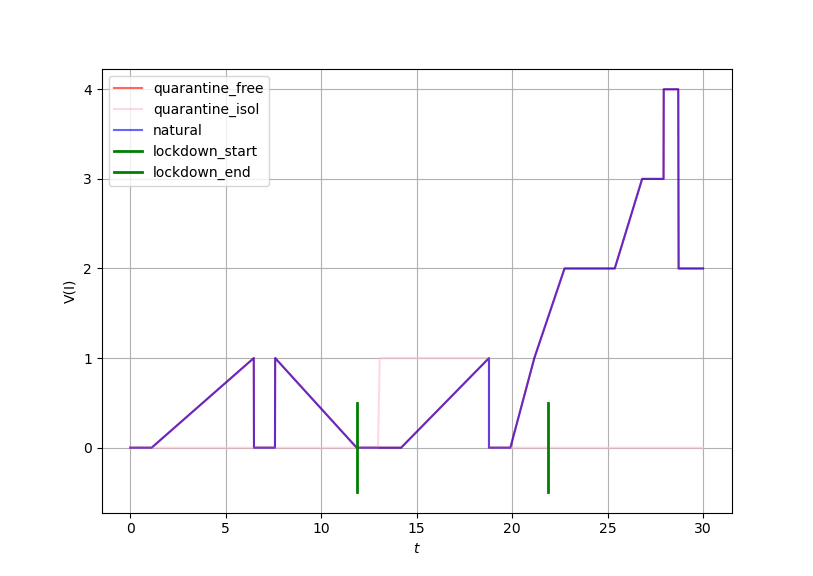
\includegraphics[width=0.8\linewidth, keepaspectratio]{../figs/basic_experiment_small_population}
		\caption{Небольшая популяция}
	\end{figure}
	
	\begin{figure}[h]
		\centering
		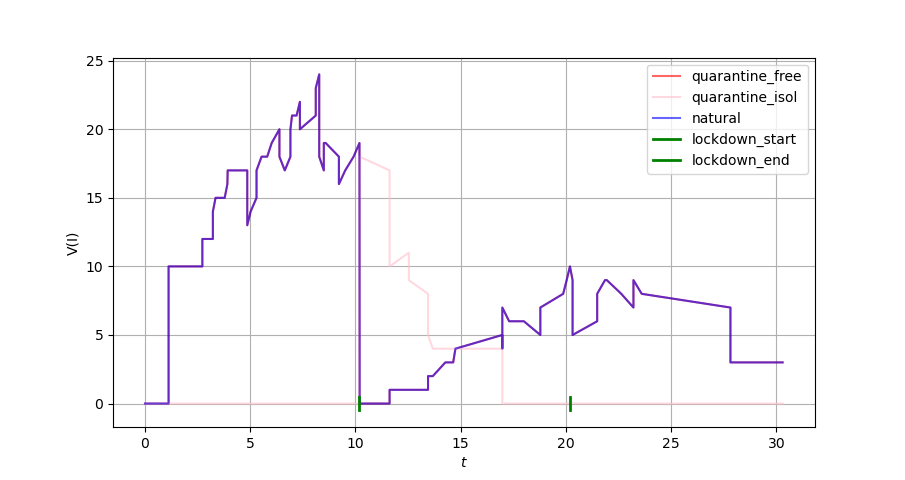
\includegraphics[width=0.8\linewidth, keepaspectratio]{../figs/basic_experiment_medium_population.png}
		\caption{Средняя популяция}
	\end{figure}
	
	\begin{figure}[h]
		\centering
		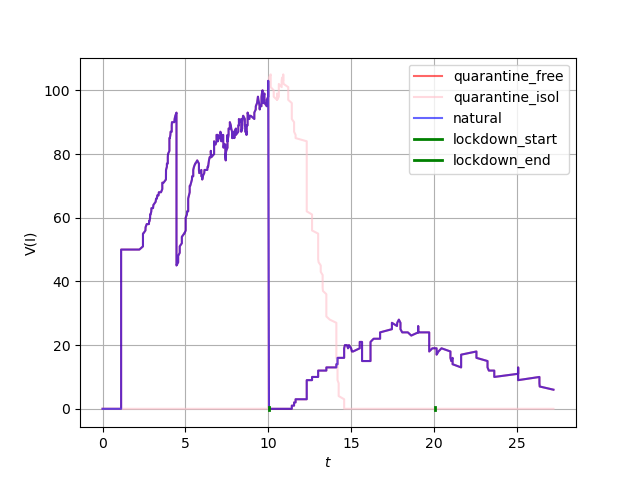
\includegraphics[width=0.8\linewidth, keepaspectratio]{../figs/basic_experiment_big_population.png}
		\caption{Большая популяция}
	\end{figure}

	% evidence 1
	\begin{figure}[h]
		\begin{center}
			\begin{minipage}{0.49\linewidth}
				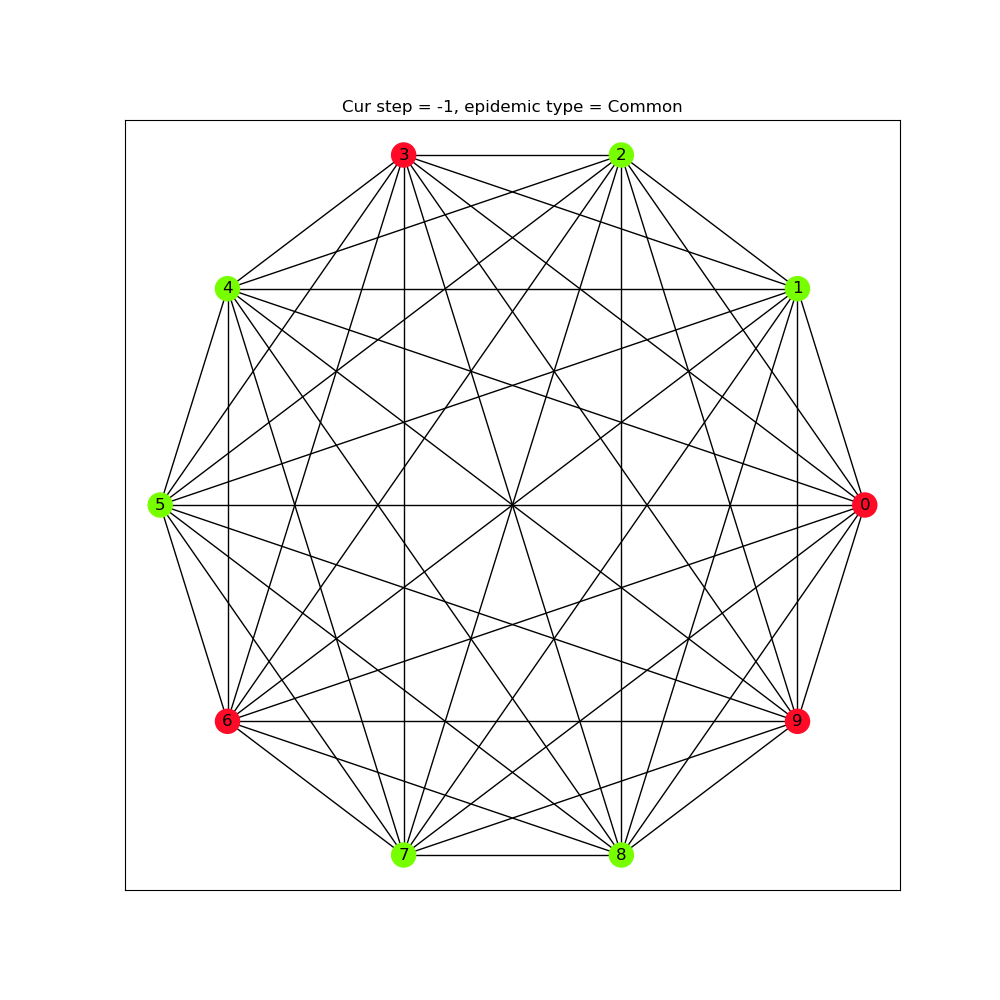
\includegraphics[width=\linewidth, keepaspectratio]{../figs/evidence2/init}
				
				\centering
				Начальная конфигурация вершин и вид <<рабочего>> графа
			\end{minipage}
			\begin{minipage}{0.49\linewidth}
				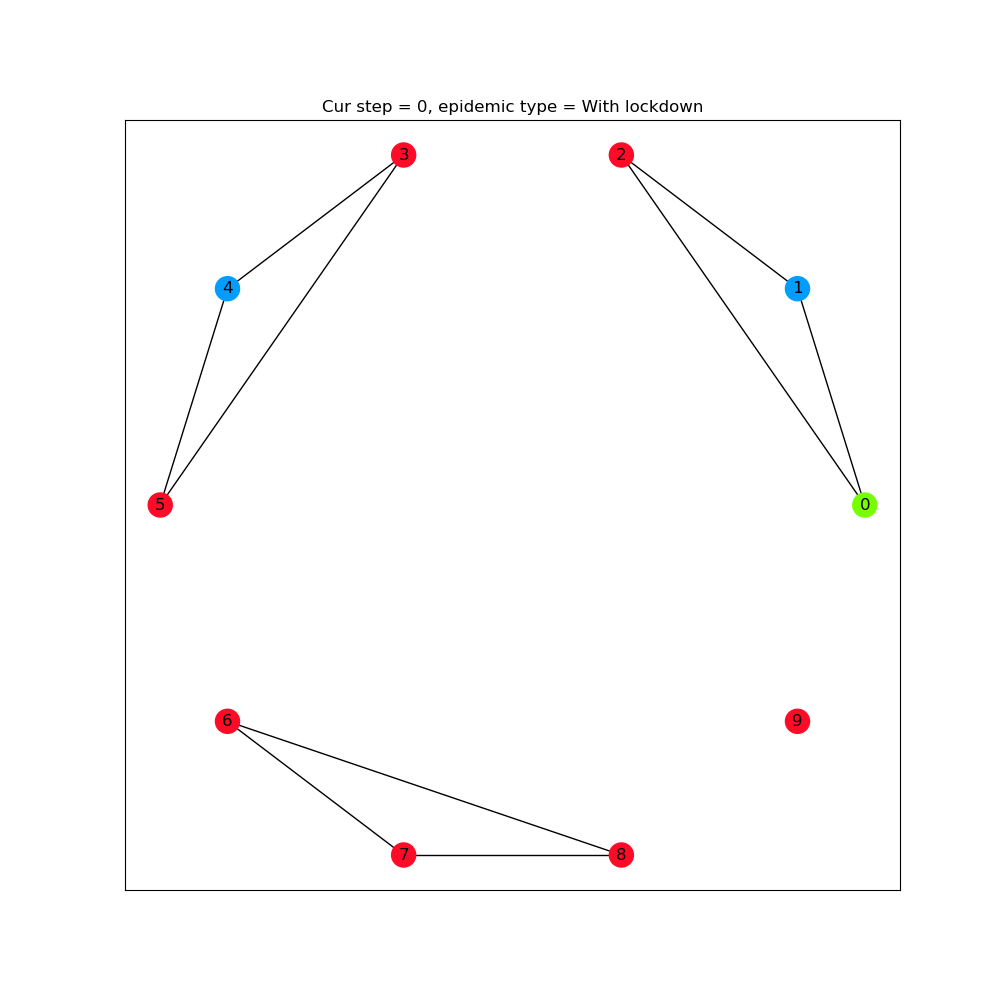
\includegraphics[width=\linewidth, keepaspectratio]{../figs/evidence2/start_with_ld}
				
				\centering
				Вид <<домашнего>> графа
			\end{minipage}
		\end{center}
		
		\begin{center}
			\begin{minipage}{0.8\linewidth}
				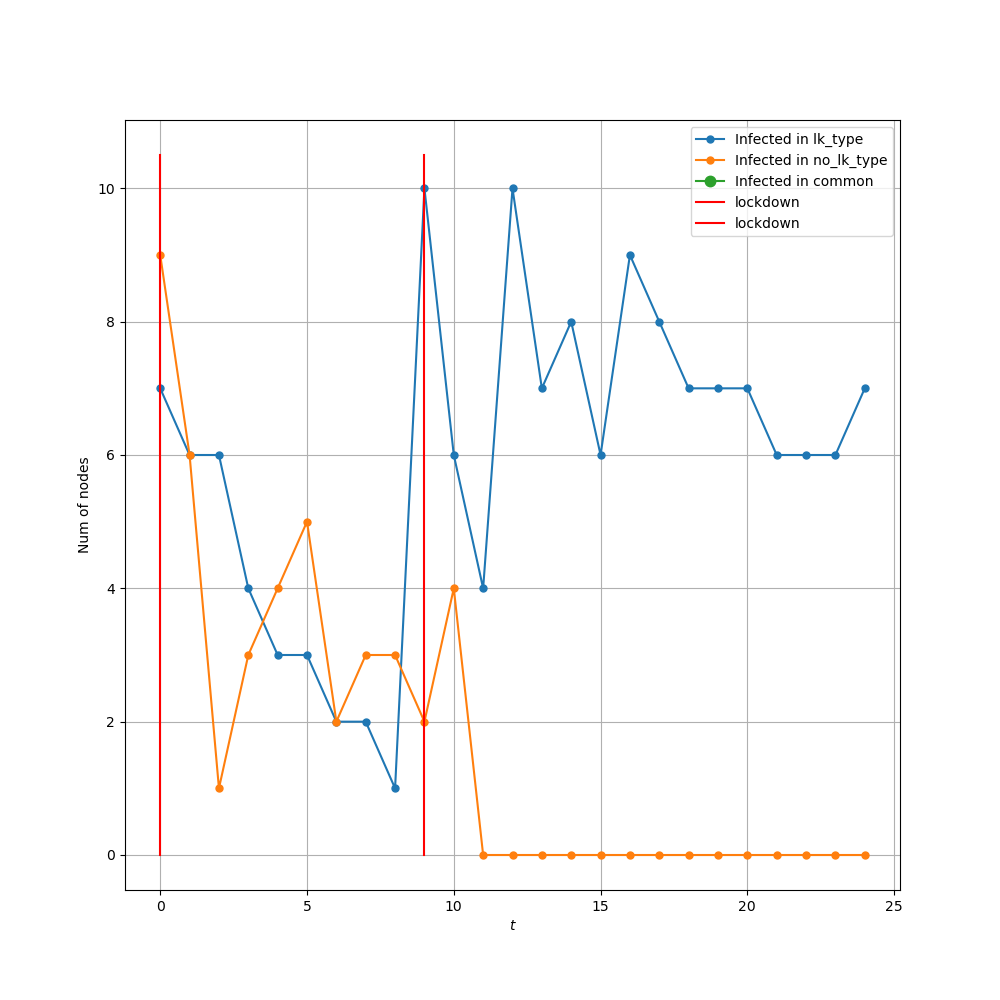
\includegraphics[width=\linewidth, keepaspectratio]{../figs/evidence2/tracks}
				
				\centering
				Сравнительные треки эпидемии с локдауном и без него
			\end{minipage}
		\end{center}
		
		\caption{Визуализация протекания эпидемии для полносвязанного графа}\label{pic:evidence_1}
	\end{figure}
	
	% evidence 2
	\begin{figure}[h]
		\begin{center}
			\begin{minipage}{0.49\linewidth}
				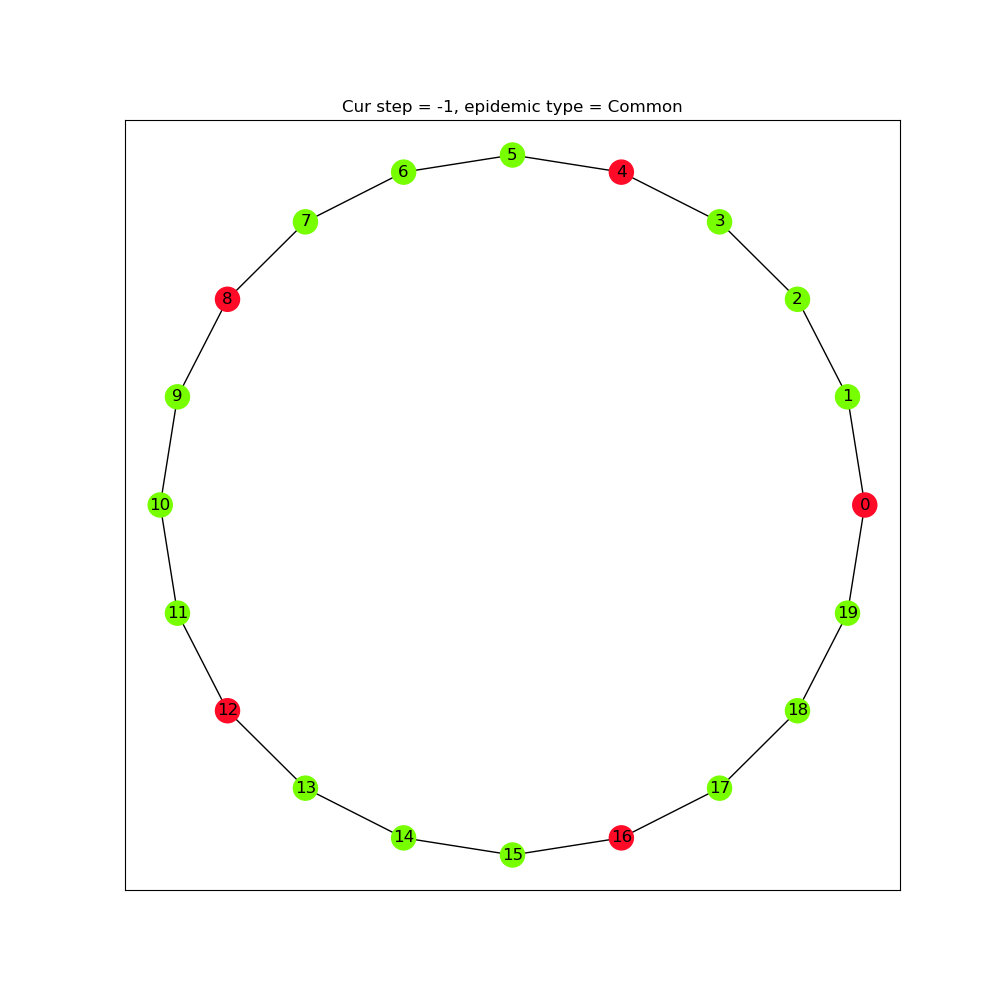
\includegraphics[width=\linewidth, keepaspectratio]{../figs/evidence3/init}
				
				\centering
				Начальная конфигурация вершин и вид <<рабочего>> графа
			\end{minipage}
			\begin{minipage}{0.49\linewidth}
				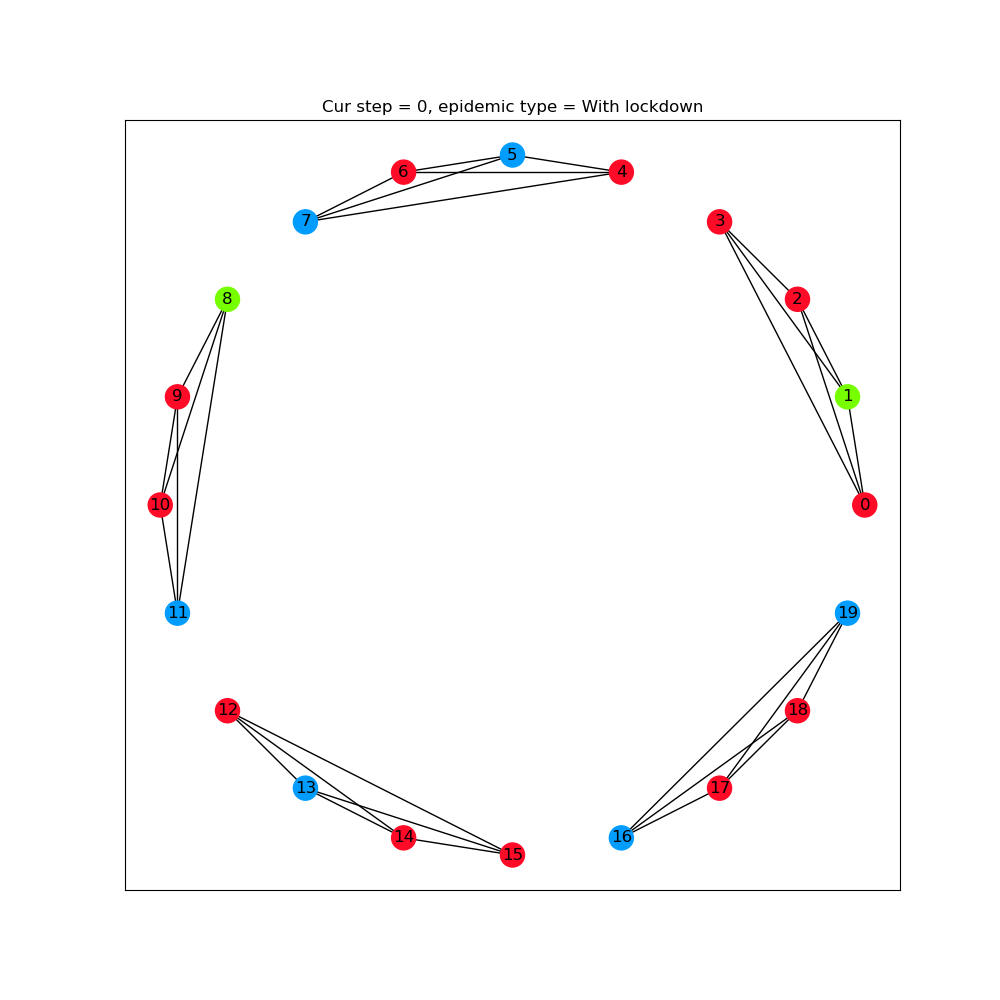
\includegraphics[width=\linewidth, keepaspectratio]{../figs/evidence3/start_with_ld}
				
				\centering
				Вид <<домашнего>> графа
			\end{minipage}
		\end{center}
		
		\begin{center}
			\begin{minipage}{0.8\linewidth}
				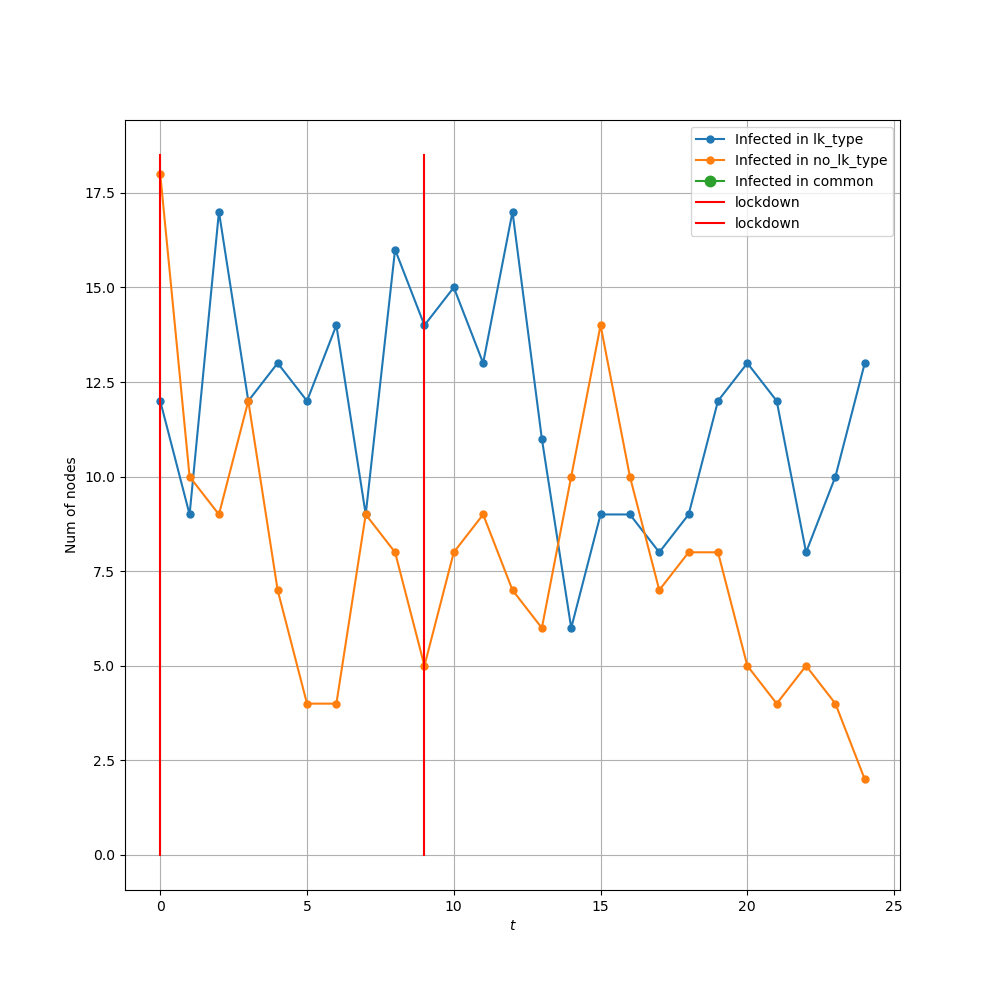
\includegraphics[width=\linewidth, keepaspectratio]{../figs/evidence3/tracks}
				
				\centering
				Сравнительные треки эпидемии с локдауном и без него
			\end{minipage}
		\end{center}
		
		\caption{Визуализация протекания эпидемии для графа-цикла}\label{pic:evidence_2}
	\end{figure}
	
\end{document}